% Op icon: N-gon prism — small hex profile, arrow, larger hex outline (the same
% profile+arrow+result pattern as extrude.tex). Two earlier attempts at an
% overlapping front/back hexagon pair (linking all 6 corners, then just the west/
% east anchors, then hand-picked "tangent" vertices) all produced stray triangular
% slivers or fully-occluded connectors — the tangent-vertex geometry for two
% congruent hexagons translated diagonally is fiddlier than it looks. This
% non-overlapping layout sidesteps the problem entirely and was verified clean.
\documentclass[tikz,border=2mm]{standalone}
\usetikzlibrary{arrows.meta,calc,shapes.geometric}
\begin{document}
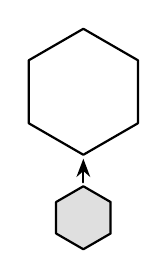
\begin{tikzpicture}[line width=1.3pt, line cap=round, line join=round, >=Stealth, x=1mm,y=1mm]
  \draw[thick, fill=gray!25] (0,-5) -- (-3.46,-7) -- (-3.46,-11) -- (0,-13) -- (3.46,-11) -- (3.46,-7) -- cycle;
  \draw[->, thick] (0,-4.5) -- (0,-1.5);
  \draw[thick] (0,15) -- (-6.93,11) -- (-6.93,3) -- (0,-1) -- (6.93,3) -- (6.93,11) -- cycle;
\end{tikzpicture}
\end{document}
